% !TEX root = ./default.tex
\maketitle

\begin{frame}
  \frametitle{목차}
  \tableofcontents
\end{frame}

\section{엔진: Tectonic}

\begin{frame}[c]
  \frametitle{\TeX{} 생태계}
  \centering
  \begin{tikzpicture}[
    node distance = 0.5cm,
    auto,
    box/.style={rectangle, draw, rounded corners, align=center},
    arrow/.style={->, >=stealth'}
  ]

    \node[box] (engines) {
      엔진\\
      \TeX,
      ε-\TeX,
      pdf\TeX,
      \XeTeX,
      \LuaTeX,
      \cemph{Tectonic}
    };

    \node[box, above = of engines] (macros) {
      매크로 패키지\\
      plain \TeX,
      \LaTeX(2ε/3),
      Con\TeX{}t
    };

    \node[box, above = of macros] (kotex) {
      상위의 패키지\\
      \koTeX,
      \AmS-\LaTeX,
      Ti$k$Z/\textsc{pgf}
    };

    \node[box, above = of kotex] (dist) {
      배포판\\
      \TeX\ Live,
      MiK\TeX,
      Mac\TeX,
      Tiny\TeX
    };

    \draw[arrow] (engines) -- (macros);
    \draw[arrow] (macros) -- (kotex);
    \draw[arrow] (kotex) -- (dist);
  \end{tikzpicture}
\end{frame}

\begin{frame}[c]
  \frametitle{Tectonic은\ldots}

  \begin{itemize}
    \item<1-> \XeTeX을 기반으로 한 \TeX{} 엔진
      \begin{itemize}
        \item 2016년에 \XeTeX에서 포크
        \item 모던 폰트와 유니코드를 지원
      \end{itemize}

    \item<1-> \TeX{} Live 배포판 사용
      \begin{itemize}
        \item 패키지들을 필요에 따라 다운로드
      \end{itemize}

    \item<2-> 러스트(Rust)로 작성
      \begin{itemize}
        \item 메모리 안전성을 보장하는 프로그래밍 언어
      \end{itemize}

    \item<3-> 멋있는 이름: τέκτων (tektōn)
      \begin{itemize}
        \item 목수
      \end{itemize}

    \item<3-> 거인의 어깨 위에
      \begin{itemize}
        \item \TeX, \LaTeX, \XeTeX, xdvipdfmx
      \end{itemize}
  \end{itemize}
\end{frame}

\begin{frame}[c]
  \frametitle{러스트?}

  \begin{itemize}
    \item<1-> 2010년 Mozilla에서 개발 시작
    \begin{itemize}
      \item 타입 수준에서 메모리 안전성을 보장
      \item C/C++과 (거의) 동일한 성능
    \end{itemize}

    \item<2-> \XeTeX: WEB2C로 생성된 C 코드를 재구성
      \begin{itemize}
        \item Tectonic은 이를 Rust로 다시 작성해나가는 중
      \end{itemize}

    \item<2-> 러스트가 지원하는 웹어셈블리(WASM)도 지원할 수 있는 가능성

    \item<3-> 러스트 crate(라이브러리)로서, 다른 프로그램에 임베딩 가능

    \item<3-> 러스트의 훌륭한 CLI와 프로젝트 구성을 계승
      \begin{itemize}
        \item \texttt{cargo} 스타일의 \texttt{tectonic} CLI 명령어
        \item 기본적으로 텍 소스와 조판된 문서를 분리하고, 텍 소스도 프리앰블과 본문 등으로 분리
      \end{itemize}
  \end{itemize}
\end{frame}

\begin{frame}[c]
  \frametitle{러스트의 친절한 CLI}

  \centering
  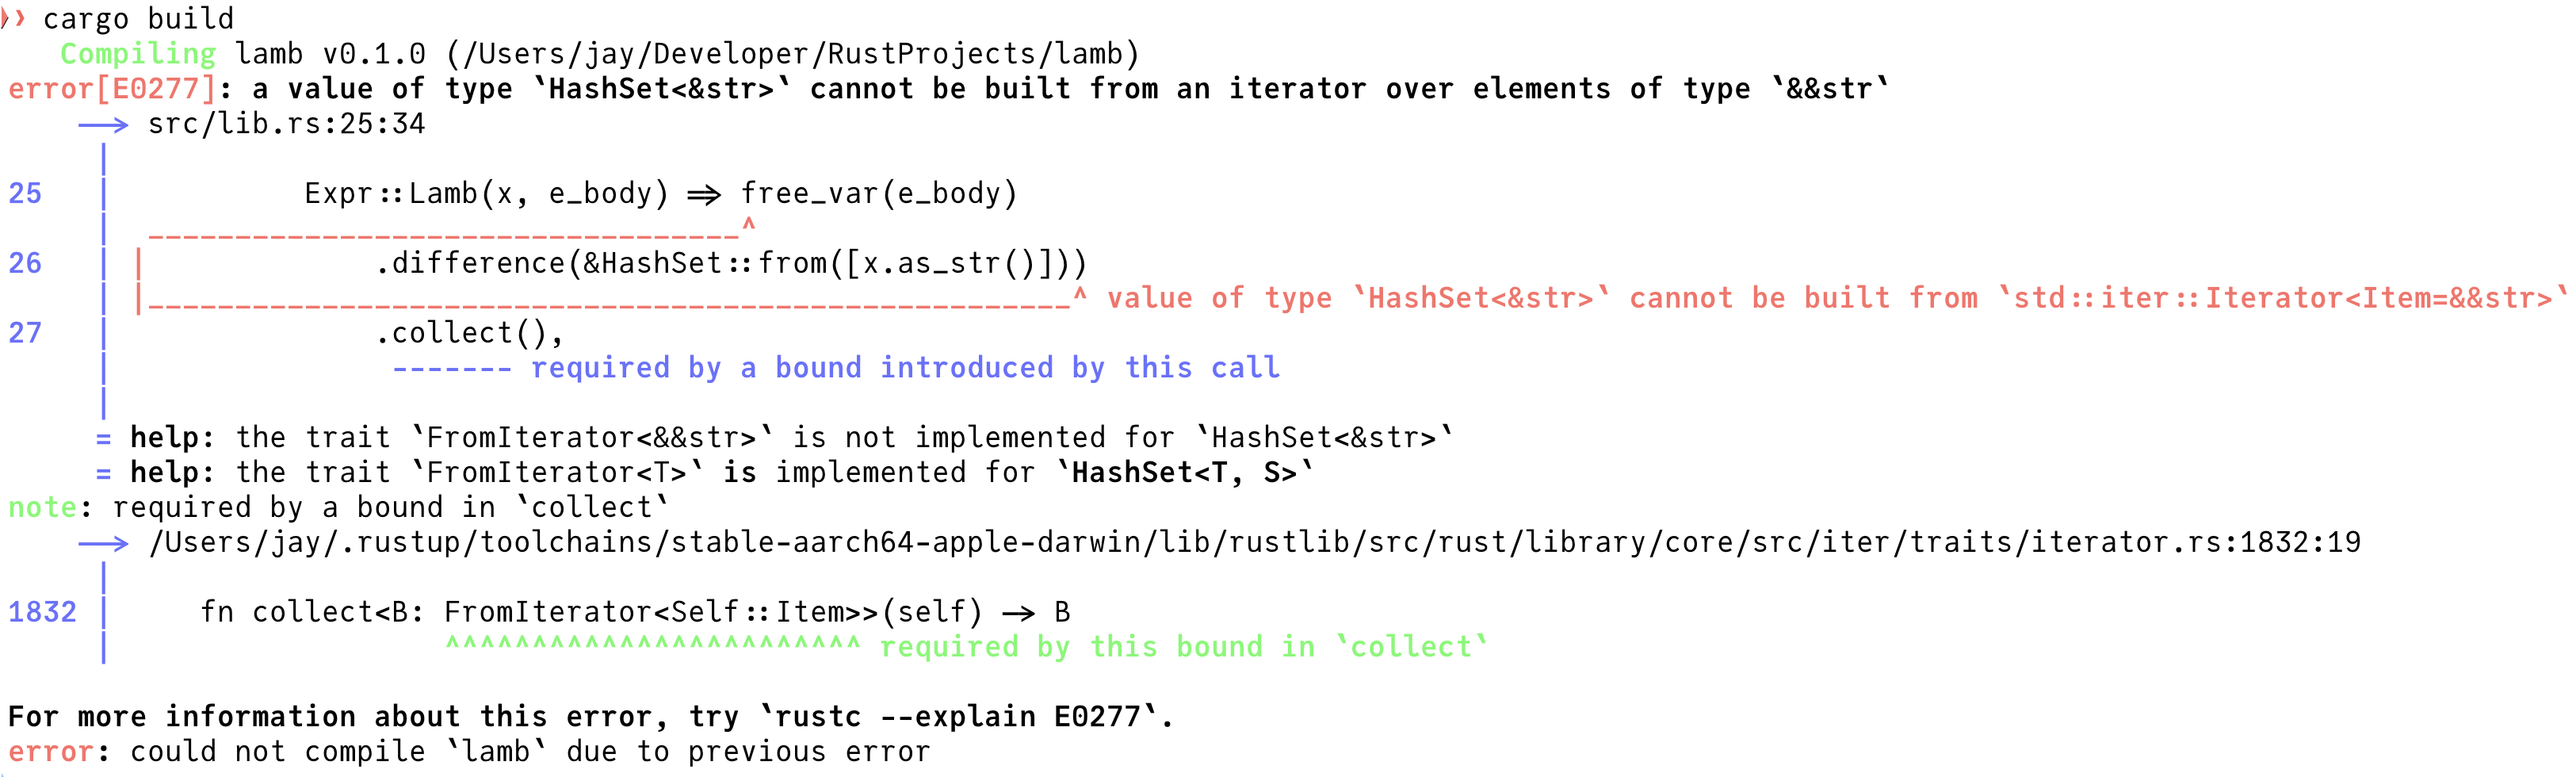
\includegraphics[width=0.8\linewidth]{cargo-cli.png}

  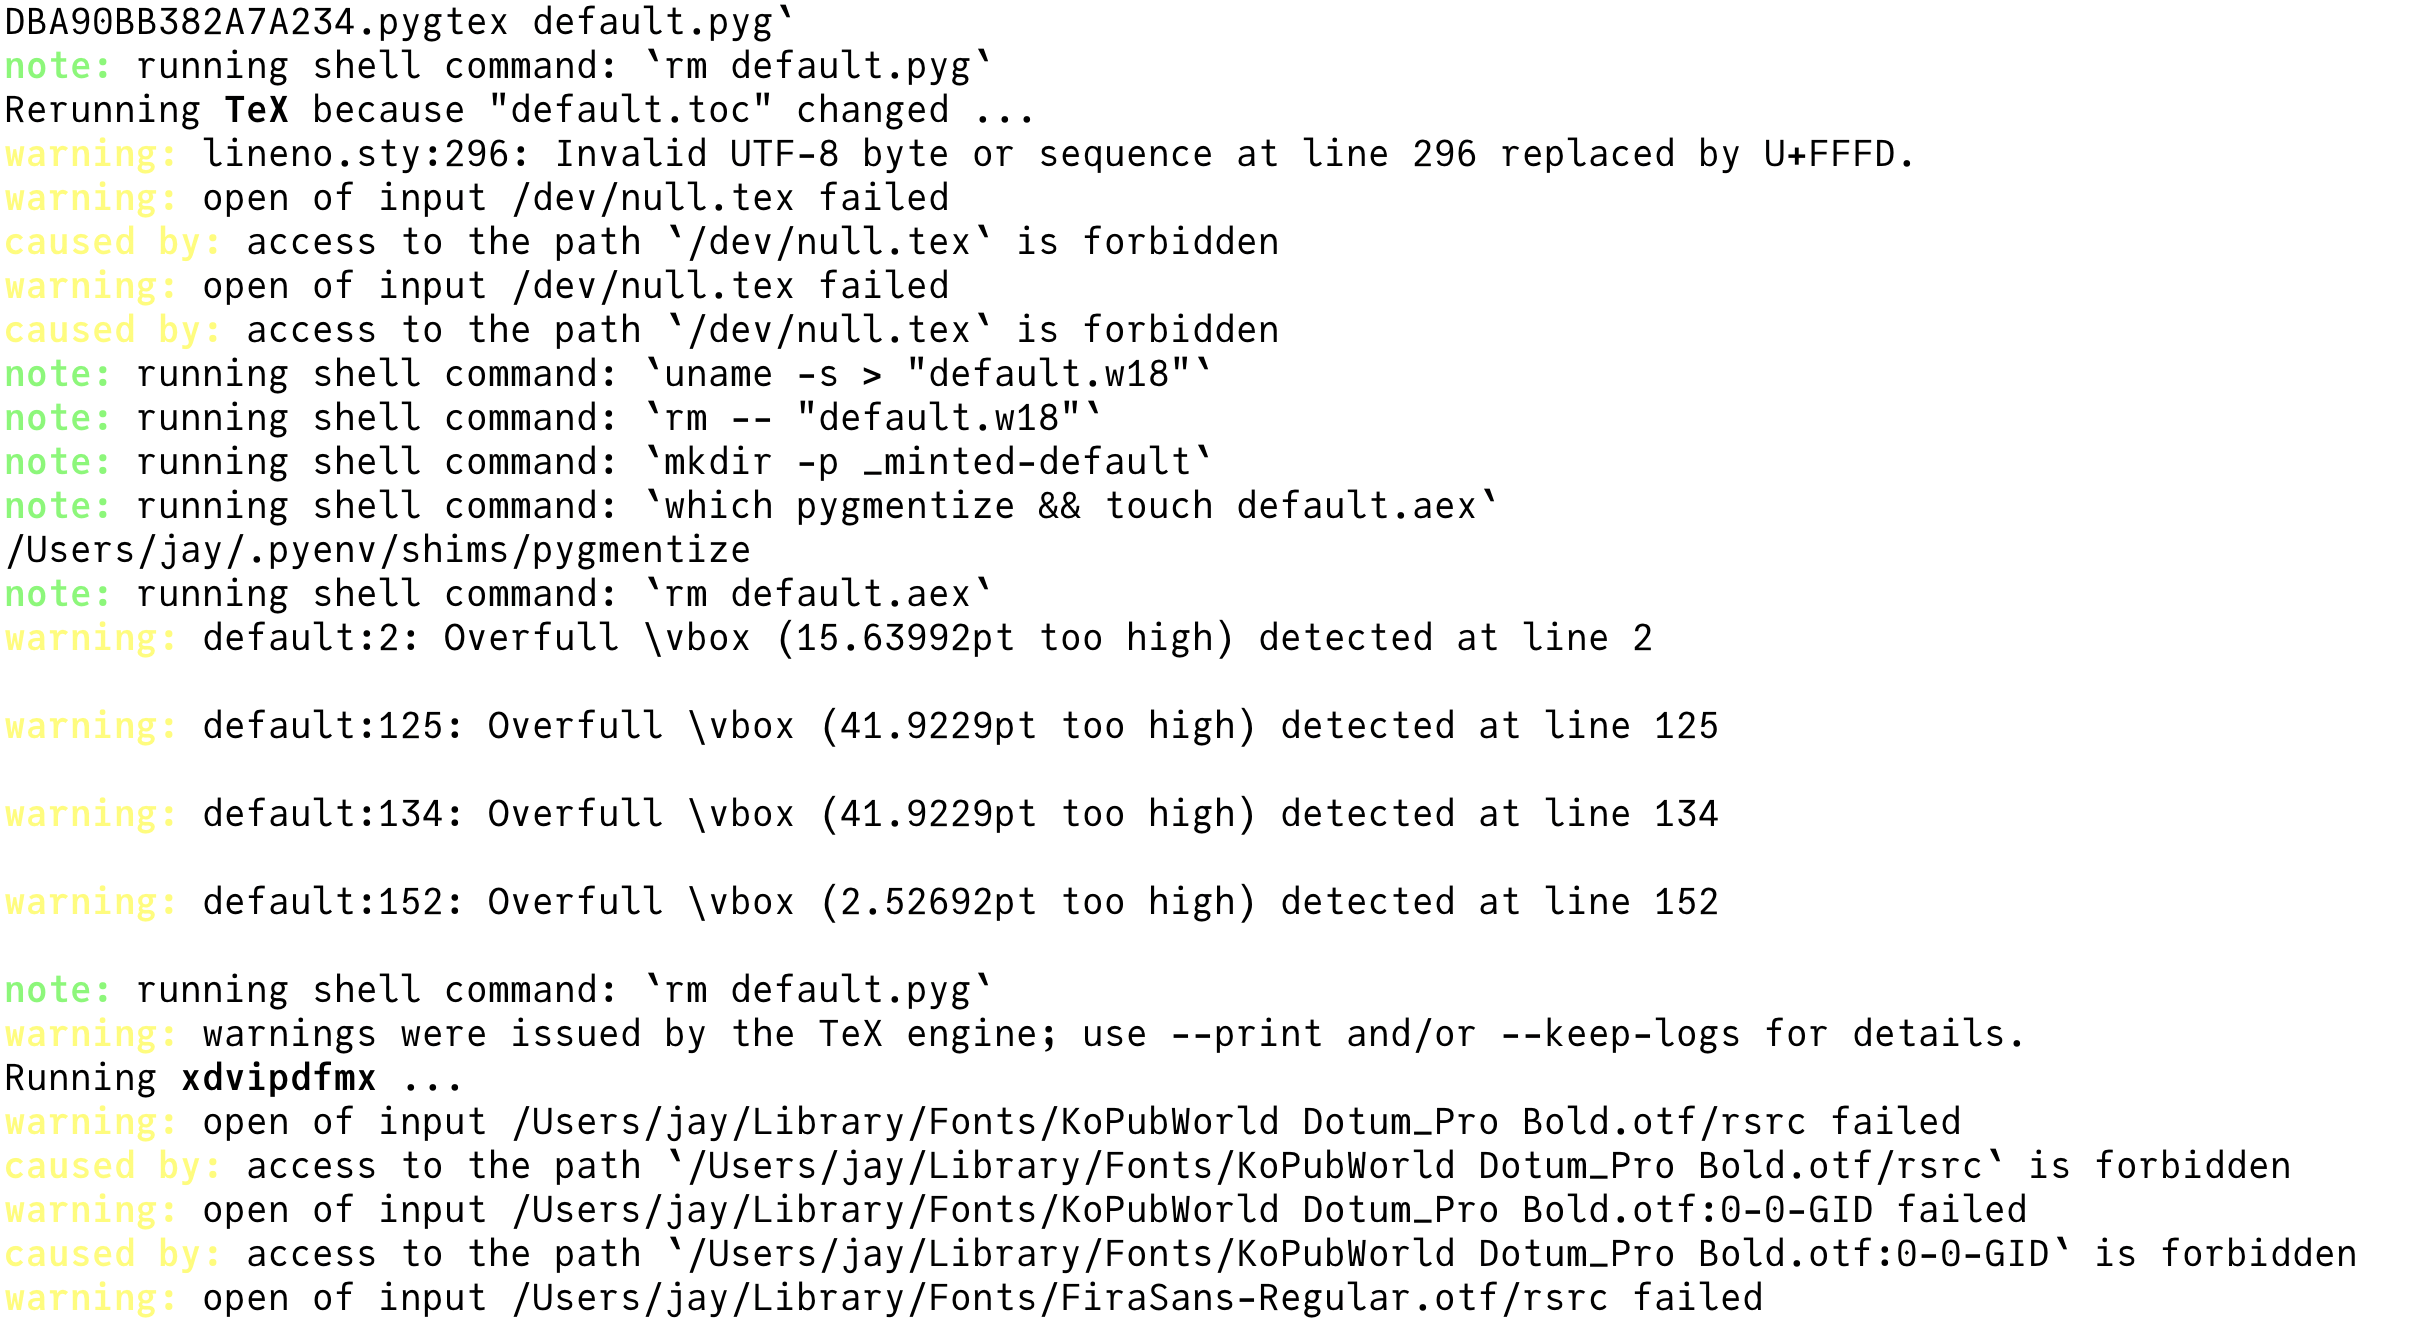
\includegraphics[width=0.8\linewidth]{tectonic-cli.png}
\end{frame}

\begin{frame}[c,fragile]
  \frametitle{사용법}

  \verb/tectonic -X/로 V2 인터페이스 사용

  \begin{itemize}
    \item \verb/tectonic -X new hello-tectonic/으로 새 프로젝트 생성
    \item \verb/cd hello-tectonic/ 후
    \item \verb/tectonic -X build/로 문서 조판
      \begin{itemize}
        \item 변경 사항이 없으면 조판하지 않음
      \end{itemize}
  \end{itemize}

  예시:
  \begin{center}
    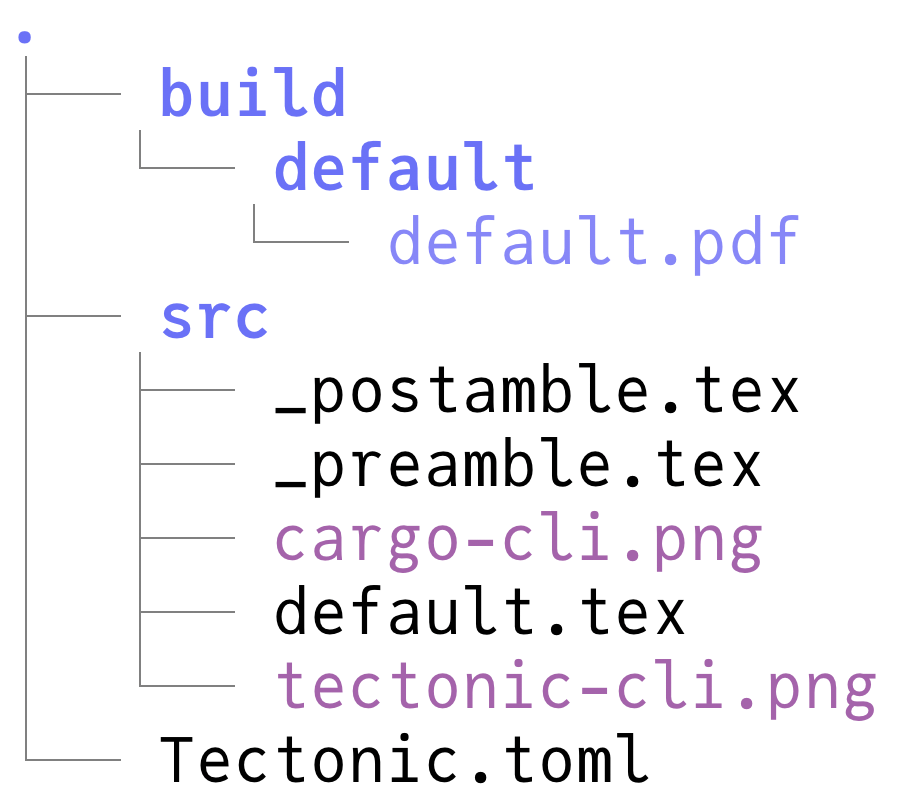
\includegraphics[width=0.4\linewidth]{tree.png}
  \end{center}
\end{frame}

\begin{frame}[c,fragile]
  \frametitle{설정 파일}
  \verb/Tectonic.toml/ (TOML 포맷)
  \begin{tomlcode}
[doc]
name = <string>
bundle = <url or filesystem path>

[[output]]
name = <string>
type = <"pdf">
tex_format = [string]
shell_escape = [bool]
preamble = [string]
index = [string]
postamble = [string]
  \end{tomlcode}
\end{frame}

\begin{frame}[c,fragile,allowframebreaks]
  \frametitle{Visual Studio Code 연동}
  LaTeX Workshop 확장과 함께 사용
  \begin{itemize}
    \item \href{https://marketplace.visualstudio.com/items?itemName=James-Yu.latex-workshop}{LaTeX Workshop} 확장을 설치
    \item \keys{\ctrl + \shift + p} (macOS: \keys{\cmd + \shift + p})로 명령 팔레트 열어서 \verb/Preferences: Open User Settings (JSON)/ 입력

    \framebreak
    \item \verb/settings.json/ 파일에 다음과 같이 추가:
    \begin{jsoncode}
  "latex-workshop.latex.recipe.default": "tectonic",
  "latex-workshop.latex.autoBuild.run": "onSave",
  "latex-workshop.latex.outDir": "%WORKSPACE_FOLDER%/build/default",
  "latex-workshop.view.pdf.viewer": "tab",
  "latex-workshop.latex.recipes": [
    {
      "name": "tectonic",
      "tools": ["tectonic"]
    }
  ],
  "latex-workshop.latex.tools": [
    {
      "name": "tectonic",
      "command": "tectonic",
      "args": ["-X", "build"],
      "env": {}
    }
  ]
    \end{jsoncode}

    \framebreak
    \item \verb/Tectonic.toml/ 파일에 다음과 같이 변경:
  \begin{tomlcode}
[[output]]
name = 'default'
index = 'default'
  \end{tomlcode}

    \item \verb/default.tex/ 첫 줄에 다음과 같이 추가:
      \verb\% !TEX root = ./default.tex\

  \end{itemize}

  참고: \url{https://github.com/tectonic-typesetting/tectonic/discussions/896#discussioncomment-6073309}
\end{frame}

\begin{frame}[c,fragile]
  \frametitle{임베딩}
  \begin{rscode}
use tectonic;
let latex = r#"
\documentclass{article}
\begin{document}
Hello, world!
\end{document}
"#;
let pdf_data: Vec<u8> = tectonic::latex_to_pdf(latex)
    .expect("processing failed");
println!("Output PDF size is {} bytes", pdf_data.len());
  \end{rscode}
  \vskip-1em
  이외에도 \texttt{tectonic::XdvipdfmxEngine} 등의 엔진을 사용할 수 있음\footnote{\url{https://docs.rs/tectonic/latest/tectonic/}}
\end{frame}

\begin{frame}[c,fragile]
  \frametitle{잠재력}

  \begin{center}
    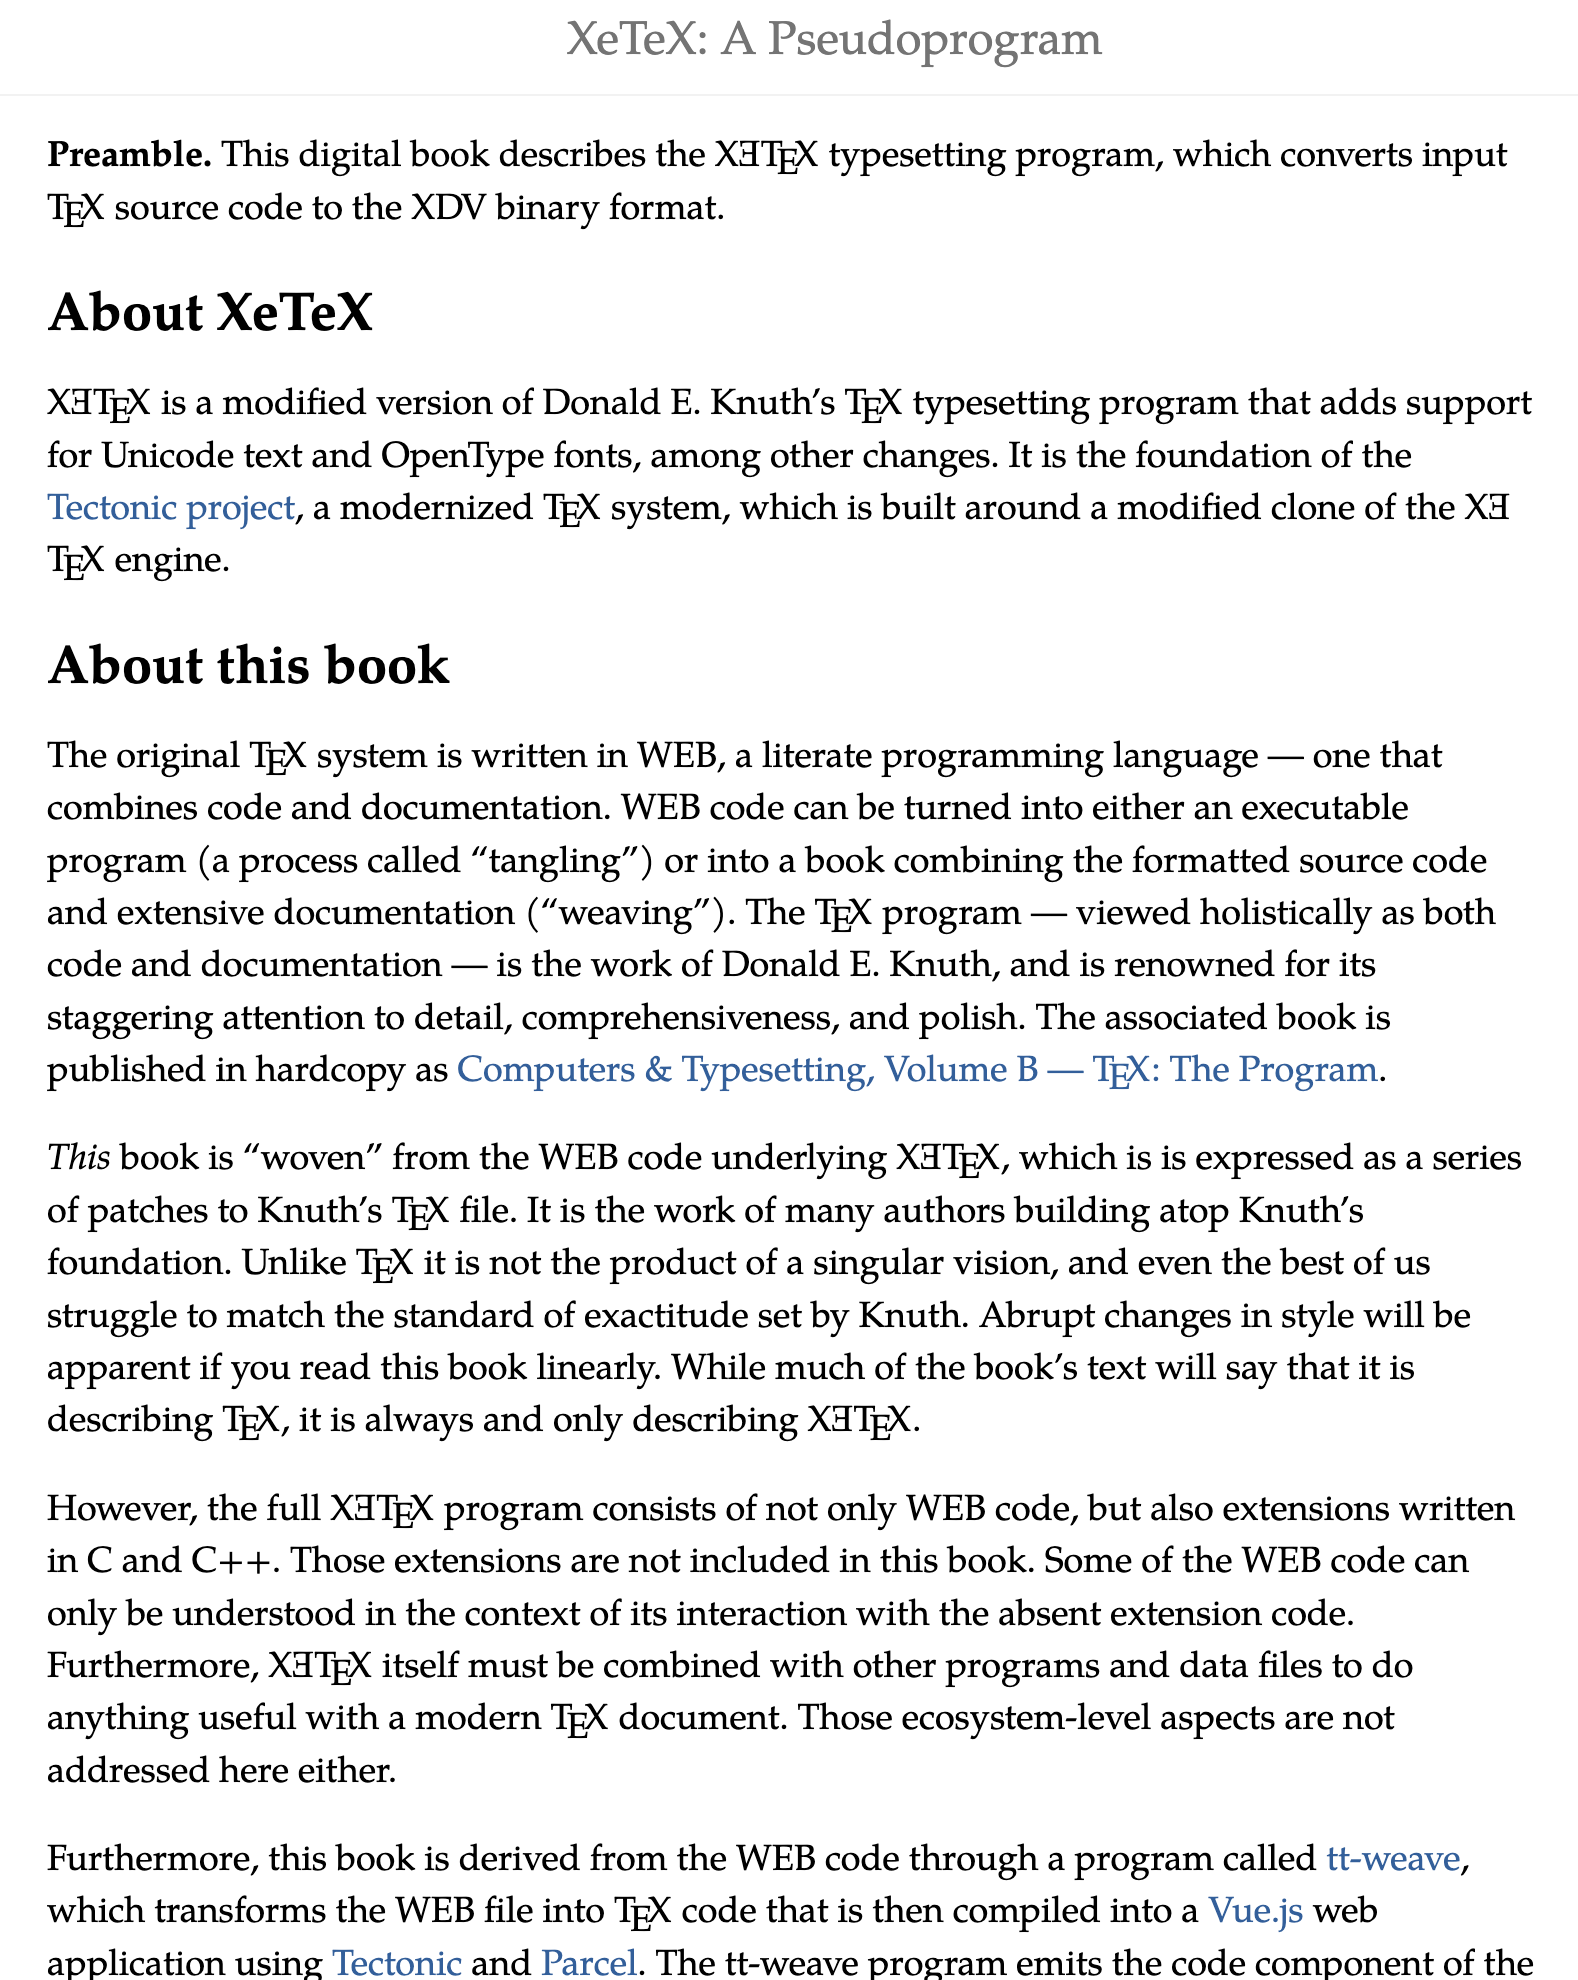
\includegraphics[width=0.5\linewidth]{xap.png}
  \end{center}
  \url{https://stacks.fullyjustified.net/xap/2022.0/#}
\end{frame}

\begin{frame}[c,fragile]
  \frametitle{한계}

  \begin{itemize}
    \item 인터넷 연결이 없다면 패키지를 다운로드할 수 없음
    \item Tectonic 프로젝트가 마지막으로 업데이트한 \TeX\ Live 버전에 의존
    \begin{itemize}
      \item 최신 버전의 패키지를 직접 CTAN에서 받아 사용해야 함
      \item \verb/src/ 디렉터리 (\verb/tectonic -X build -Z search-path=<path>/)
      \item 오버리프(Overleaf)를 사용하는 경우와 유사
    \end{itemize}
  \end{itemize}
\end{frame}

\begin{frame}[c]
  \frametitle{참고: ksminitex}

  \begin{center}
    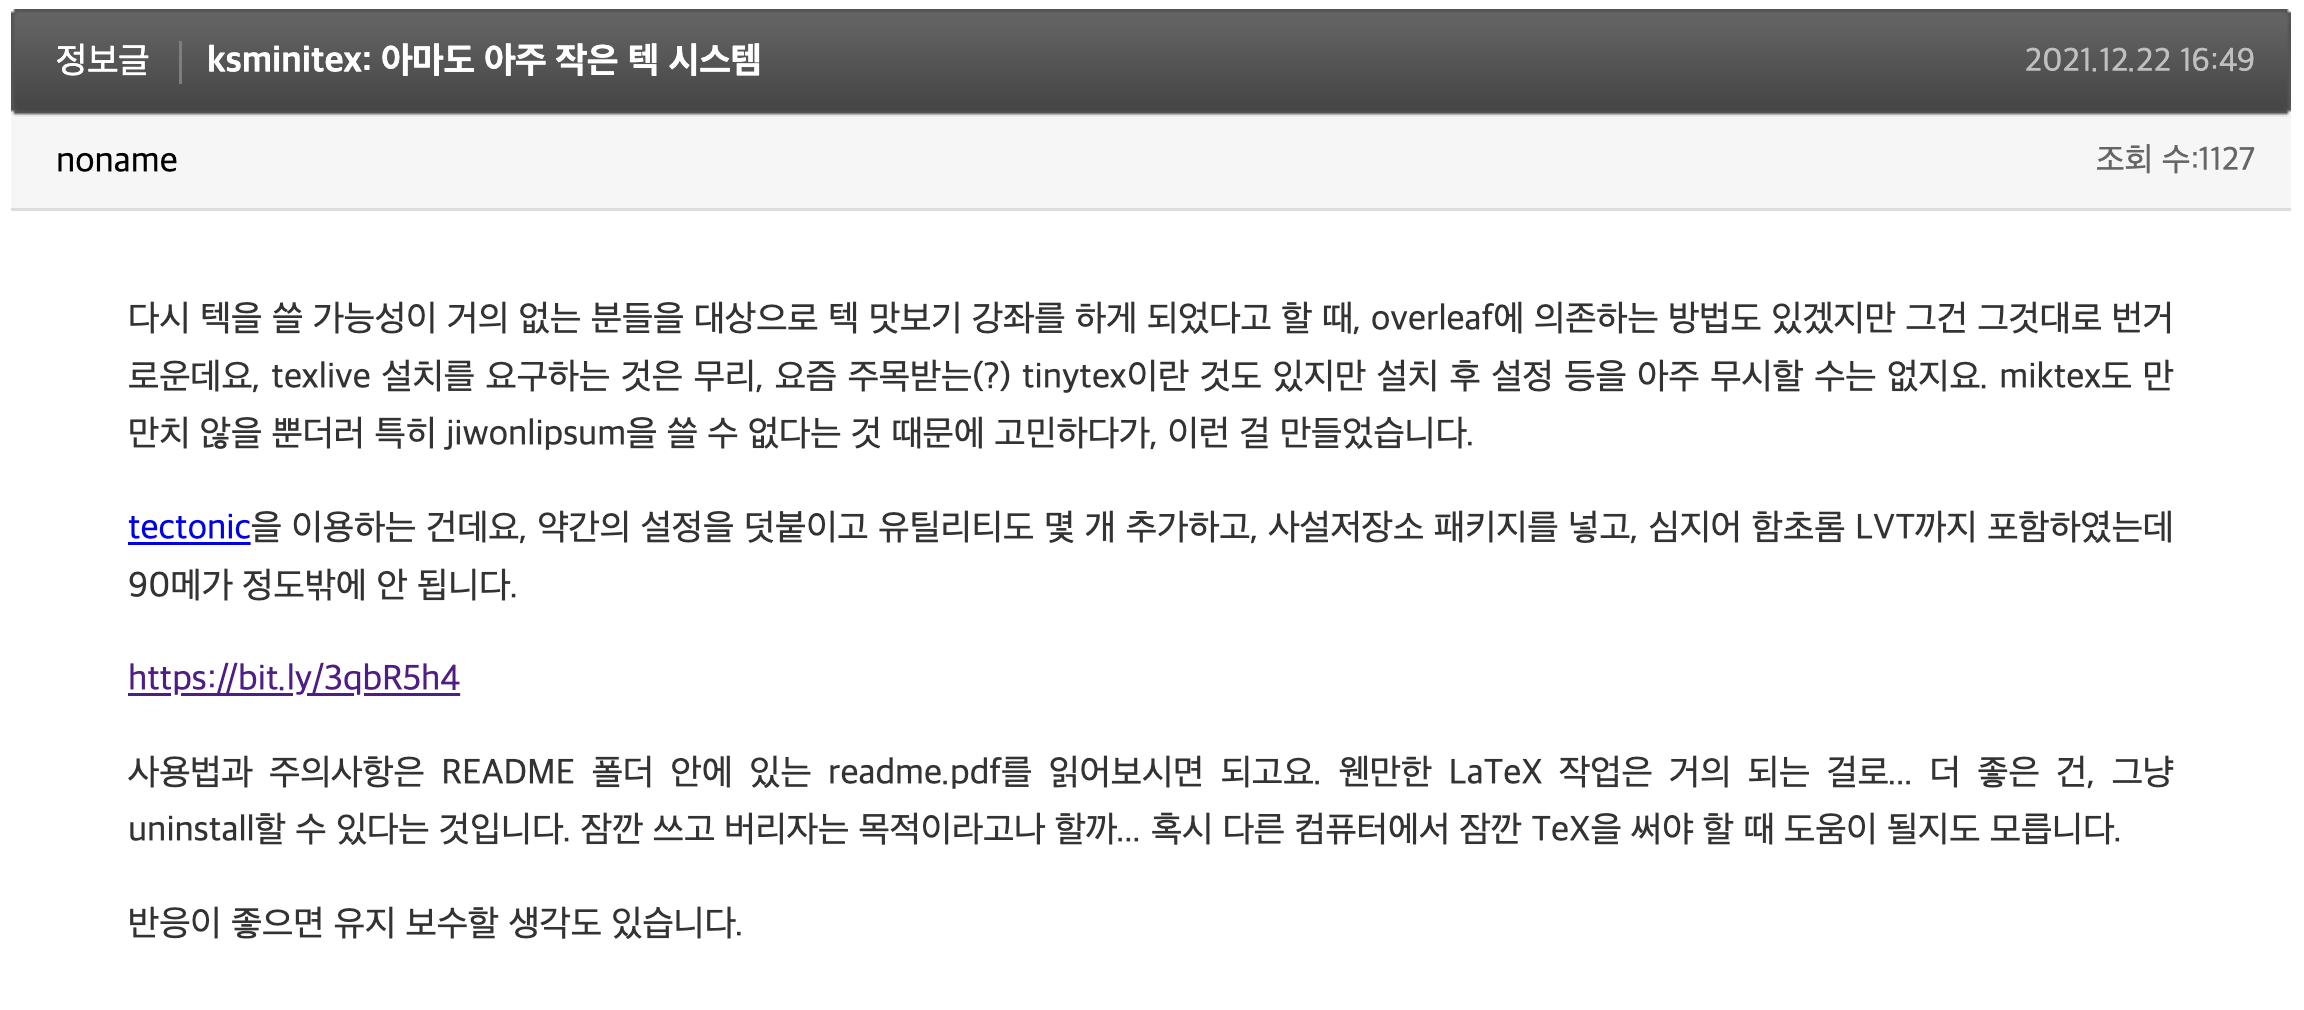
\includegraphics[width=\linewidth]{ksminitex.png}
  \end{center}
\end{frame}


\section{자동화: GitHub Actions}
\begin{frame}[c]
  \frametitle{지속적 통합 및 배포 (CI/CD)}

  \begin{itemize}
    \item 지속적 통합(Continuous Integration, CI): 코드 저장소에 변경 사항이 있을 때 자동으로 빌드 및 테스트
      \begin{itemize}
        \item 코드의 오류를 빠르게 발견하고, 코드 저장소의 코드 상태가 항상 정상인지 확인
      \end{itemize}
    \item 지속적 배포(Continuous Deployment, CD): 지속적 통합을 통해 빌드 및 테스트를 통과한 코드를 자동으로 배포
      \begin{itemize}
        \item 보다 빠르게 세상에 새로운 기능을 제공
      \end{itemize}
  \end{itemize}
\end{frame}

\begin{frame}[c]
  \frametitle{GitHub Actions}

  \begin{itemize}
    \item GitHub에서 제공하는 CI/CD 서비스
    \item GitHub 저장소에 특정 이벤트가 발생하면 자동으로 작업 수행
    \item 공개된 여러 액션들을 조합하거나 직접 액션을 만들어 원하는 작업을 수행
  \end{itemize}
\end{frame}

\begin{frame}[c]
  \frametitle{Tectonic \texttt{❤} GitHub Actions}

  TeX Live 도커 이미지를 사용하는 통상의 GitHub Action은 느릴 수 밖에 없지만,
  Tectonic은 필요한 패키지만 받아서 실행하기 때문에 훨씬 가볍고 빠름

  \url{https://github.com/xu-cheng/latex-action/issues/13}
\end{frame}

\begin{frame}[c,fragile]
  \frametitle{데모: GitHub에 푸시하면 문서를 조판}

  \texttt{./.github/workflows/tectonic.yml}
  \begin{yamlcode}
name: 'Build LaTeX Document'
on:
  push:
jobs:
  build:
    runs-on: ubuntu-latest

    steps:
      - name: Checkout
        uses: actions/checkout@v3
      - uses: wtfjoke/setup-tectonic@v2
        with:
          github-token: ${{ secrets.GITHUB_TOKEN }}
      - name: Run Tectonic
        run: tectonic -X build
      - name: Upload pdf
        uses: actions/upload-artifact@v3
        with:
          name: index
          path: build/default/default.pdf
  \end{yamlcode}
\end{frame}


\section{인공지능: ChatGPT/GitHub Copilot}
\begin{frame}[c]
  \frametitle{글글글}
  일반적으로 글을 쓰는 것은 고된 노동
  \pause
  \begin{itemize}
    \item<2-> \textbf{\LaTeX으로 문서를 작성하는 더욱 큰 노동}
      \begin{itemize}
        \item 단순히 내용이 아니라 모양에 대해서도 신경 써야 함
        \item 보기 좋은 떡이 먹기도 좋다 $\leftrightarrow$ 빛 좋은 개살구
      \end{itemize}

    \item<3-> 긴 매크로들을 입력하기 위해 필요한 손재주?
      \begin{itemize}
        \item 단축기 숙달 (Vim-fu, Emacs-fu, VSCode-fu(?!), \ldots)
        \item 스니펫 활용
        \item \TeX\ 매크로 정의
        \item<4-> \cemph{조수에게 도움 받기}
      \end{itemize}

      \item<5-> \TeX을 쓰다가 질문이 생겼을 때?
        \begin{itemize}
          \item Google-fu (Bing-fu(?!))
          \item 로컬 고수에게 질문
          \item KTUG, \TeX\ StackExchange, \ldots
          \item<6-> \cemph{조수에게 도움 받기}
        \end{itemize}
  \end{itemize}
\end{frame}

\begin{frame}[c]
  \begin{center}
    {\large
      \cemph{내용} $\leftrightarrow$ \cemphr{모양} \\
    }

    \pause
    여러 자연어 및 프로그래밍 관련 작업에 적합한 ChatGPT는 두 마리 토끼를 다,
    GitHub Copilot은 국조적인 ``자동 완성'' 수준에서 도움.
  \end{center}
\end{frame}

\begin{frame}
  \frametitle{대형 언어 모델 (\cemphr{L}arge \cemphr{L}anguage \cemphr{M}odel)}

  \begin{itemize}
    \item ChatGPT: OpenAI GPT-3.5/GPT-4
      \begin{itemize}
        \item GPT-3: 1750억, GPT-4: 1조
        \item \cemphr{플러긴 스토어 등장}
      \end{itemize}
    \item GitHub Copilot: OpenAI Codex (GPT-3)
  \end{itemize}
\end{frame}

\begin{frame}
  \frametitle{시나리오: 세미나 발표}

  \begin{enumerate}
    \item<1-> 탐색
      \begin{itemize}
        \item 브레인스토밍
        \item 문헌 조사
      \end{itemize}

    \item<2-> 구체화
      \begin{itemize}
        \item 주제 선정
        \item 개요 작성
      \end{itemize}

    \item<3-> 자료 수집 및 가공

    \item<4-> 발표 자료 작성
  \end{enumerate}
\end{frame}

\begin{frame}[c]
  \frametitle{ChatGPT 데모: 개요 작성}

  GPT-4 + Plugin Prompt Perfect

  \begin{quotation}
    perfect I need to prepare a seminar for a LaTeX workshop. The topic is "TeX in a modern computing environment: engine, automation, and AI". For the engine, I will introduce the use of Tectonic; for the automation, GitHub actions; for AI, LLM like you, ChatGPT and GitHub Copilot. Can you provide me an outline? The seminar is about 30 minutes long.
  \end{quotation}
\end{frame}

\begin{frame}[c]
  \frametitle{ChatGPT 데모: 모르는 패키지 사용}

  GPT-4 + Plugin Ask Your PDF

  \begin{quotation}
    I would like to express a BNF expression of a simple call-by-value lambda calculus using simplebnf LaTeX package. Here is the manual for it: https://mirror.kakao.com/CTAN/macros/latex/contrib/simplebnf/simplebnf-doc.pdf
  \end{quotation}

  \begin{bnfgrammar}
    e : Expressions ::=
      v : variable
    | \lambda v.e : abstraction
    | e1 e2 : application
  \end{bnfgrammar}
\end{frame}


\begin{frame}[c,fragile]
  \frametitle{GitHub Copilot 데모: 명령어 자동 완성}

  \begin{texcode}
% centered image
\begin{center}
  \includegraphics[width=\linewidth]{copilot.png}
\end{center}
  \end{texcode}

\end{frame}

% add a frame for finishing the talk
